%%%%%%%%%%%%%%%%%%%%%%%%%%%%%%%%%%%%%%%%%%%%%%%%%%%%%%%%%%%%%%
%% Chapter 3: Annotation Platform
%%%%%%%%%%%%%%%%%%%%%%%%%%%%%%%%%%%%%%%%%%%%%%%%%%%%%%%%%%%%%%

\section{Annotation Platform}
\label{chap:annotation-platform}

Sign language corpora suitable for training the models described in
Chapters~\ref{chap:isolated-gloss-recognition} and~\ref{chap:text-translation}
are scarce, which motivated building a dedicated platform for collecting and
labelling sign language video data. This chapter describes the functional
requirements, system architecture, and data format of that platform. The
platform's source code is hosted publicly on GitHub at
\url{https://github.com/stachurski2k/SLEP}, which also hosts the project board
used for work management.

\subsection{Functional requirements}
\label{sec:annotation-functional-requirements}

The main development objectives for the annotation platform were to:

\begin{itemize}
  \item build a working data collection application for sign language video
        datasets;
  \item provide dataset, video, gesture class, and gesture type management;
  \item support video upload through object storage instead of storing large
        files directly in the database;
  \item process uploaded videos asynchronously so that landmark extraction does
        not block HTTP requests;
  \item extract body, face, and hand landmarks from videos using MediaPipe;
  \item provide a browser-based editor for selecting frame ranges and saving
        annotated gesture clips;
  \item prepare the project for local development through Docker Compose.
\end{itemize}

The frontend is implemented with React~19, TypeScript, Vite, React Router,
Tailwind CSS, ESLint, and Sonner notifications. The interface uses a dark
professional theme and is organised around reusable UI components such as
tables, dialogs, navigation, and the video editor. The frontend provides several
main views, backed by the API areas listed in
Section~\ref{sec:annotation-system-architecture}:

\begin{itemize}
  \item \textbf{Video editor} -- select datasets and videos, preview the current
        video, step through frames, set clip start and end points, assign
        gesture metadata, and save clips. It loads selected videos through
        signed download URLs, displays playback controls, supports frame
        stepping, shows a timeline with zoom, stores start and end frame
        markers, and submits clip annotations to the backend. It also caches
        the selected gesture class and gesture type in local storage to reduce
        repeated manual selection during annotation work;
  \item \textbf{Dataset Manager} -- list datasets, create new datasets, delete
        datasets, and open a dataset-specific video view;
  \item \textbf{Dataset Videos view} -- list videos belonging to a dataset,
        preview selected videos, import new videos, and open videos in the
        editor;
  \item \textbf{Gesture Class management} -- maintain the list of gesture
        classes used during annotation;
  \item \textbf{Gesture Type management} -- maintain the list of gesture types
        used during annotation.
\end{itemize}

\begin{figure}[htbp]
  \centering
  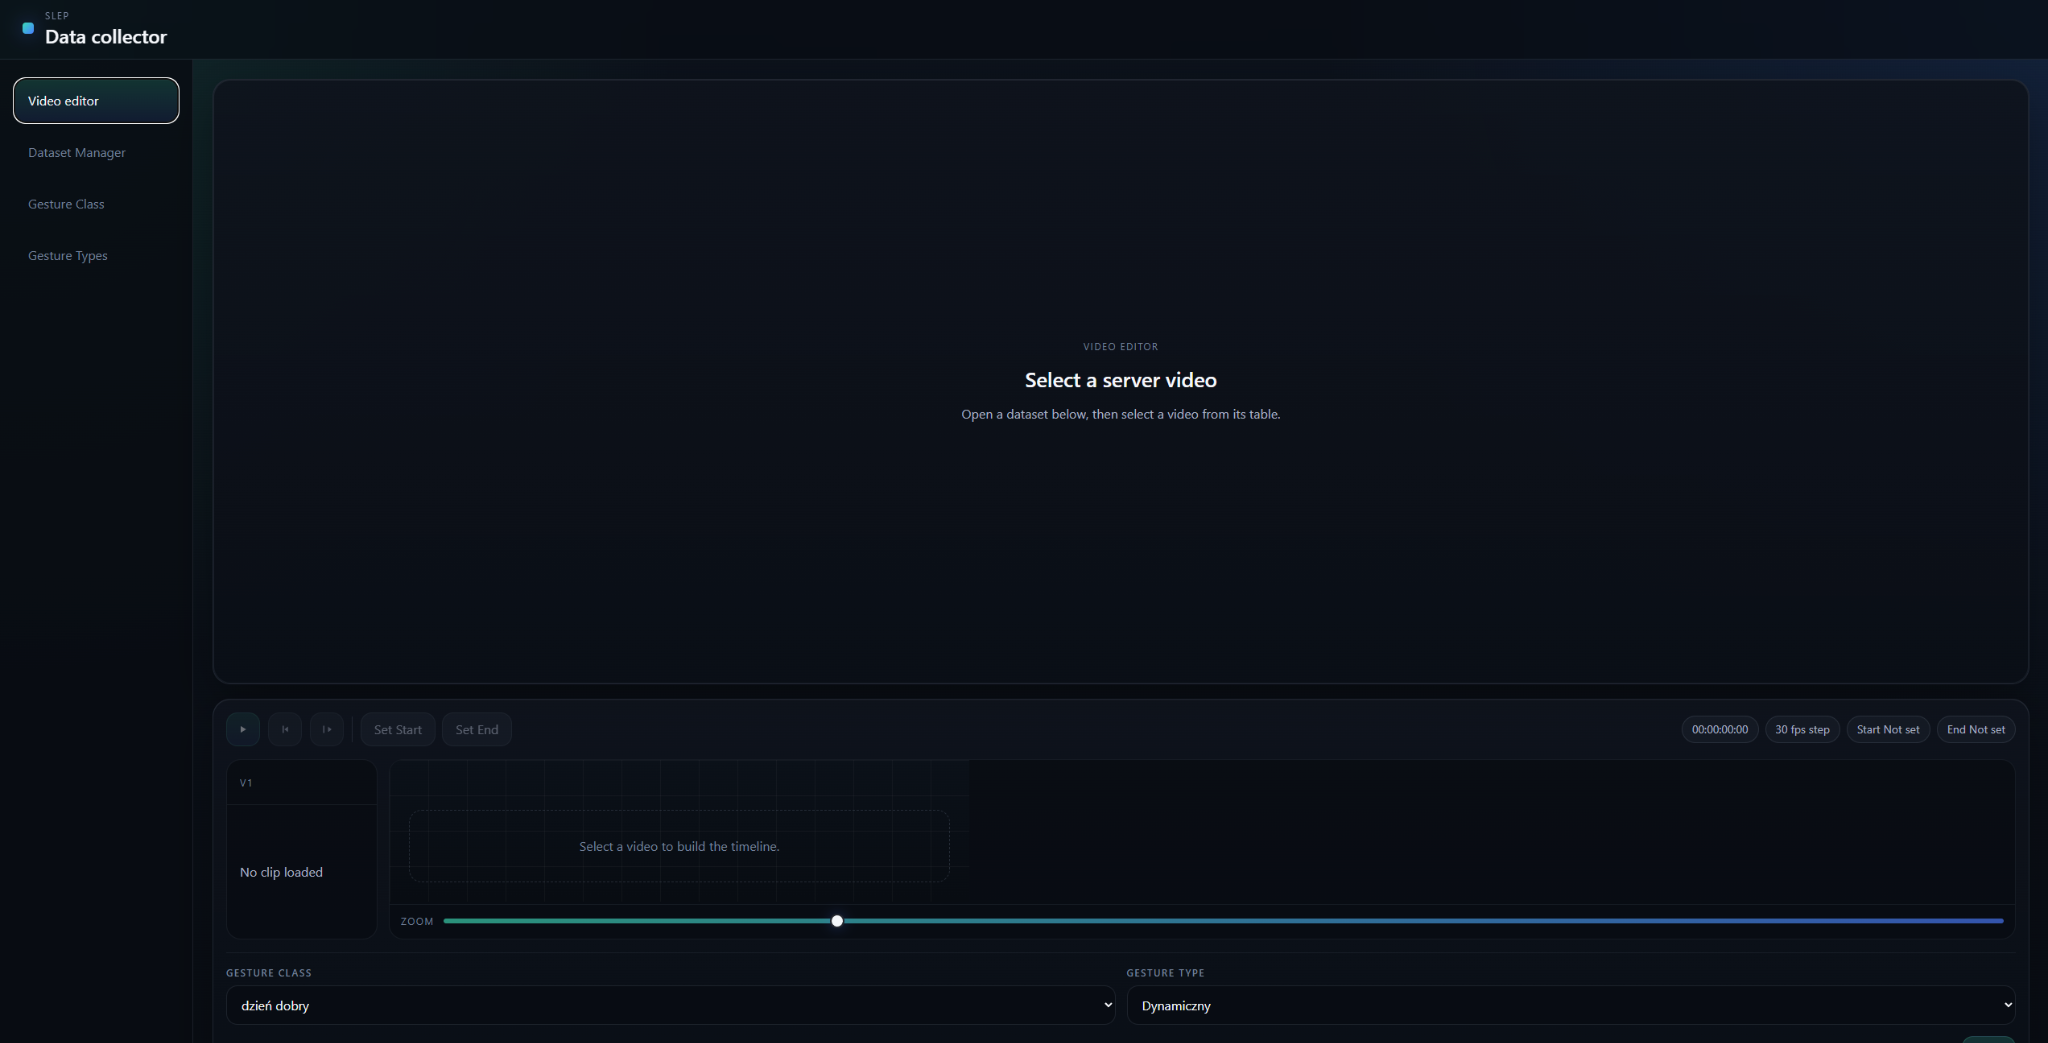
\includegraphics[width=0.85\textwidth]{figures/annotation-platform/video-editor-page.png}
  \caption{Video editor page.}
  \label{fig:video-editor-page}
\end{figure}

\begin{figure}[htbp]
  \centering
  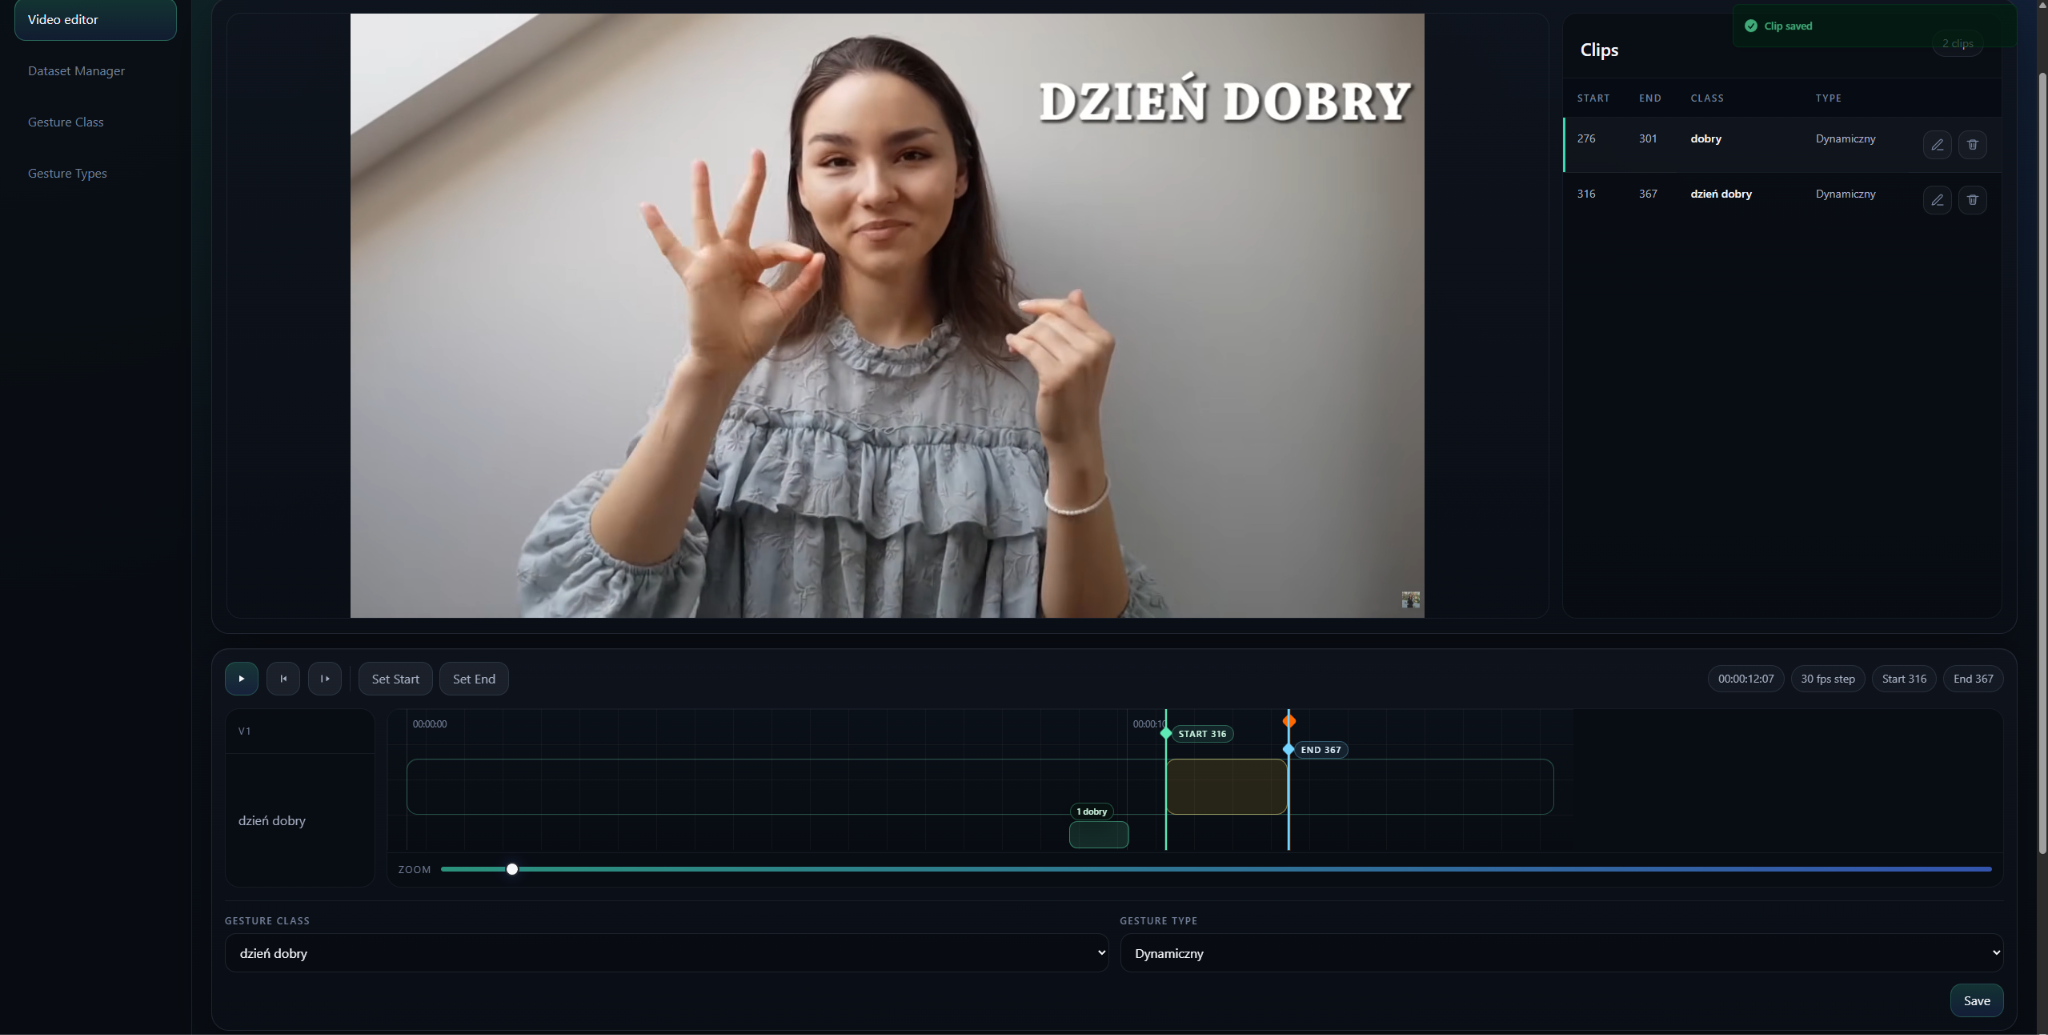
\includegraphics[width=0.85\textwidth]{figures/annotation-platform/video-editor-sample.png}
  \caption{Video editor with a sample video loaded.}
  \label{fig:video-editor-sample}
\end{figure}

\begin{figure}[htbp]
  \centering
  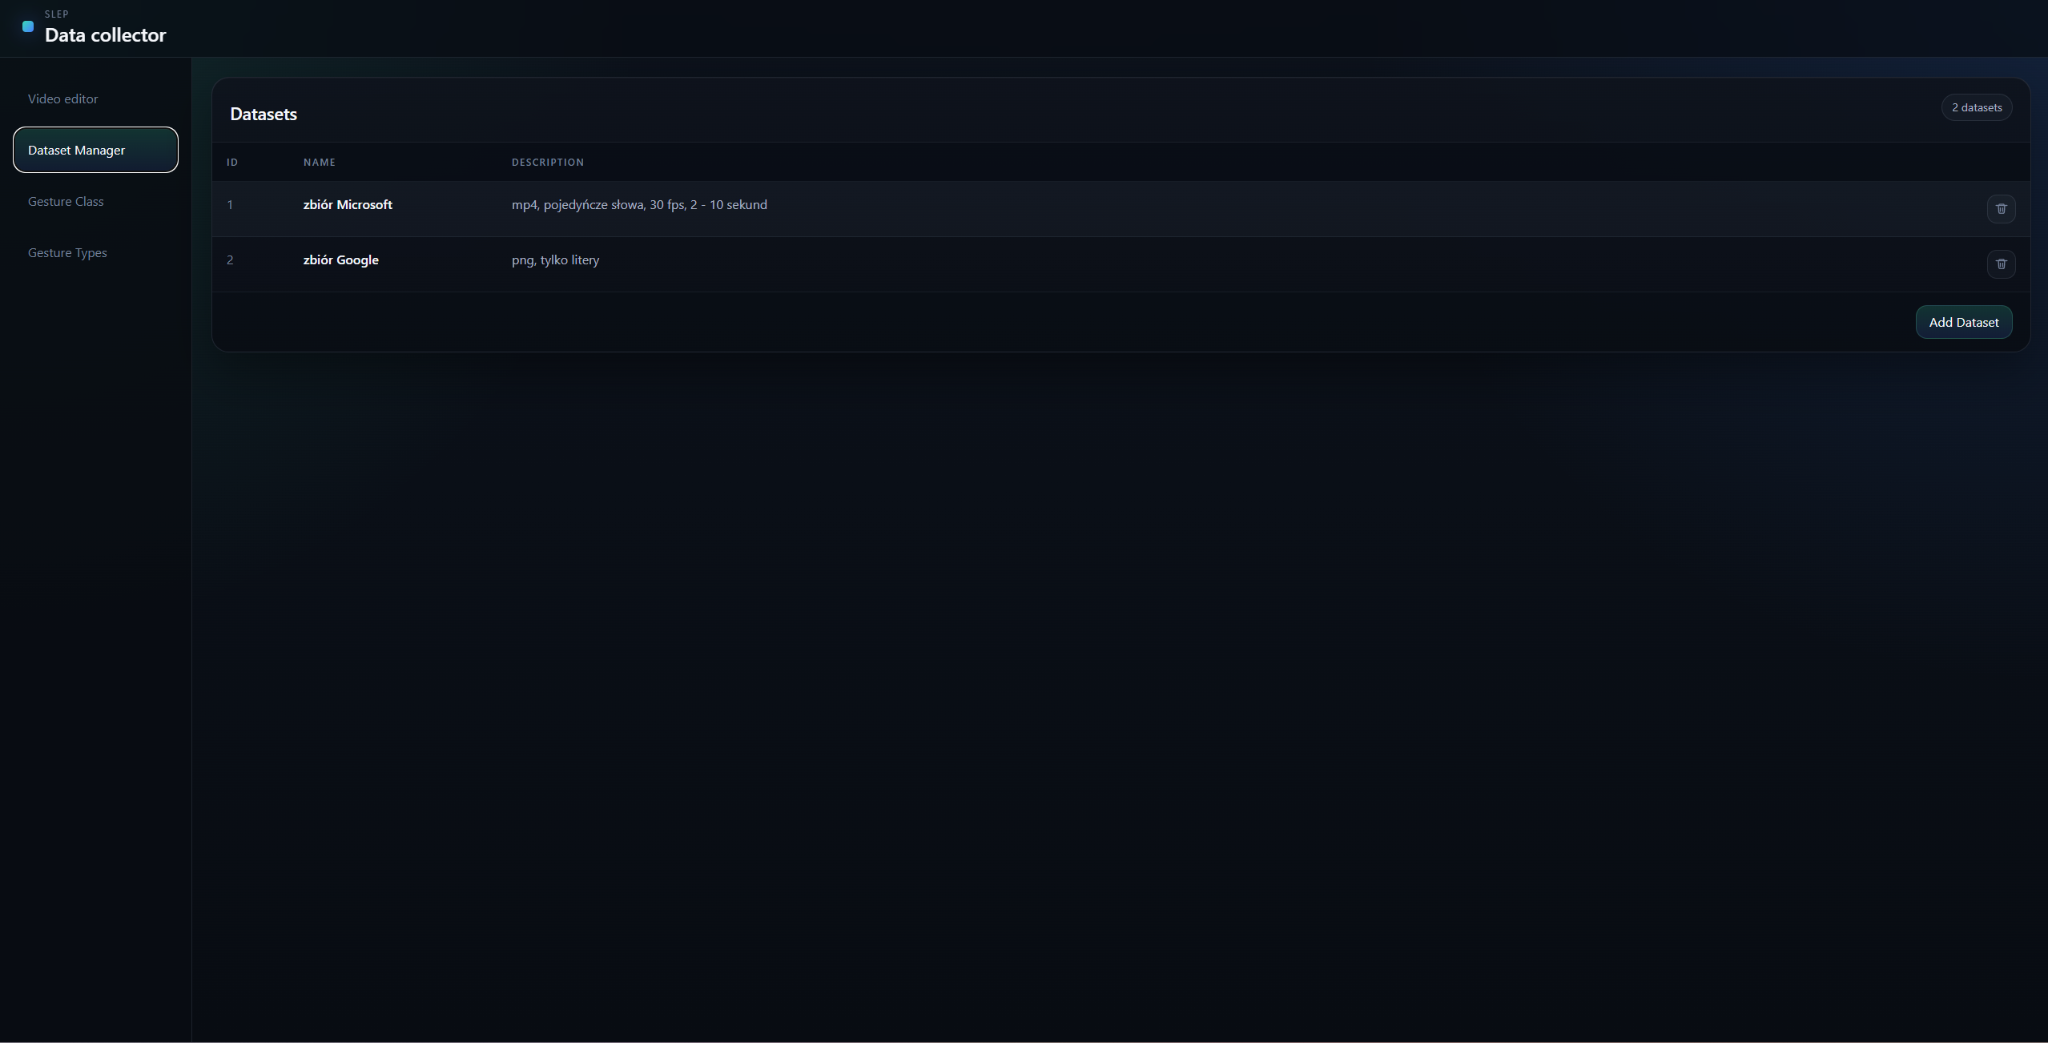
\includegraphics[width=0.7\textwidth]{figures/annotation-platform/dataset-manager-page.png}
  \caption{Dataset Manager page.}
  \label{fig:dataset-manager-page}
\end{figure}

\begin{figure}[htbp]
  \centering
  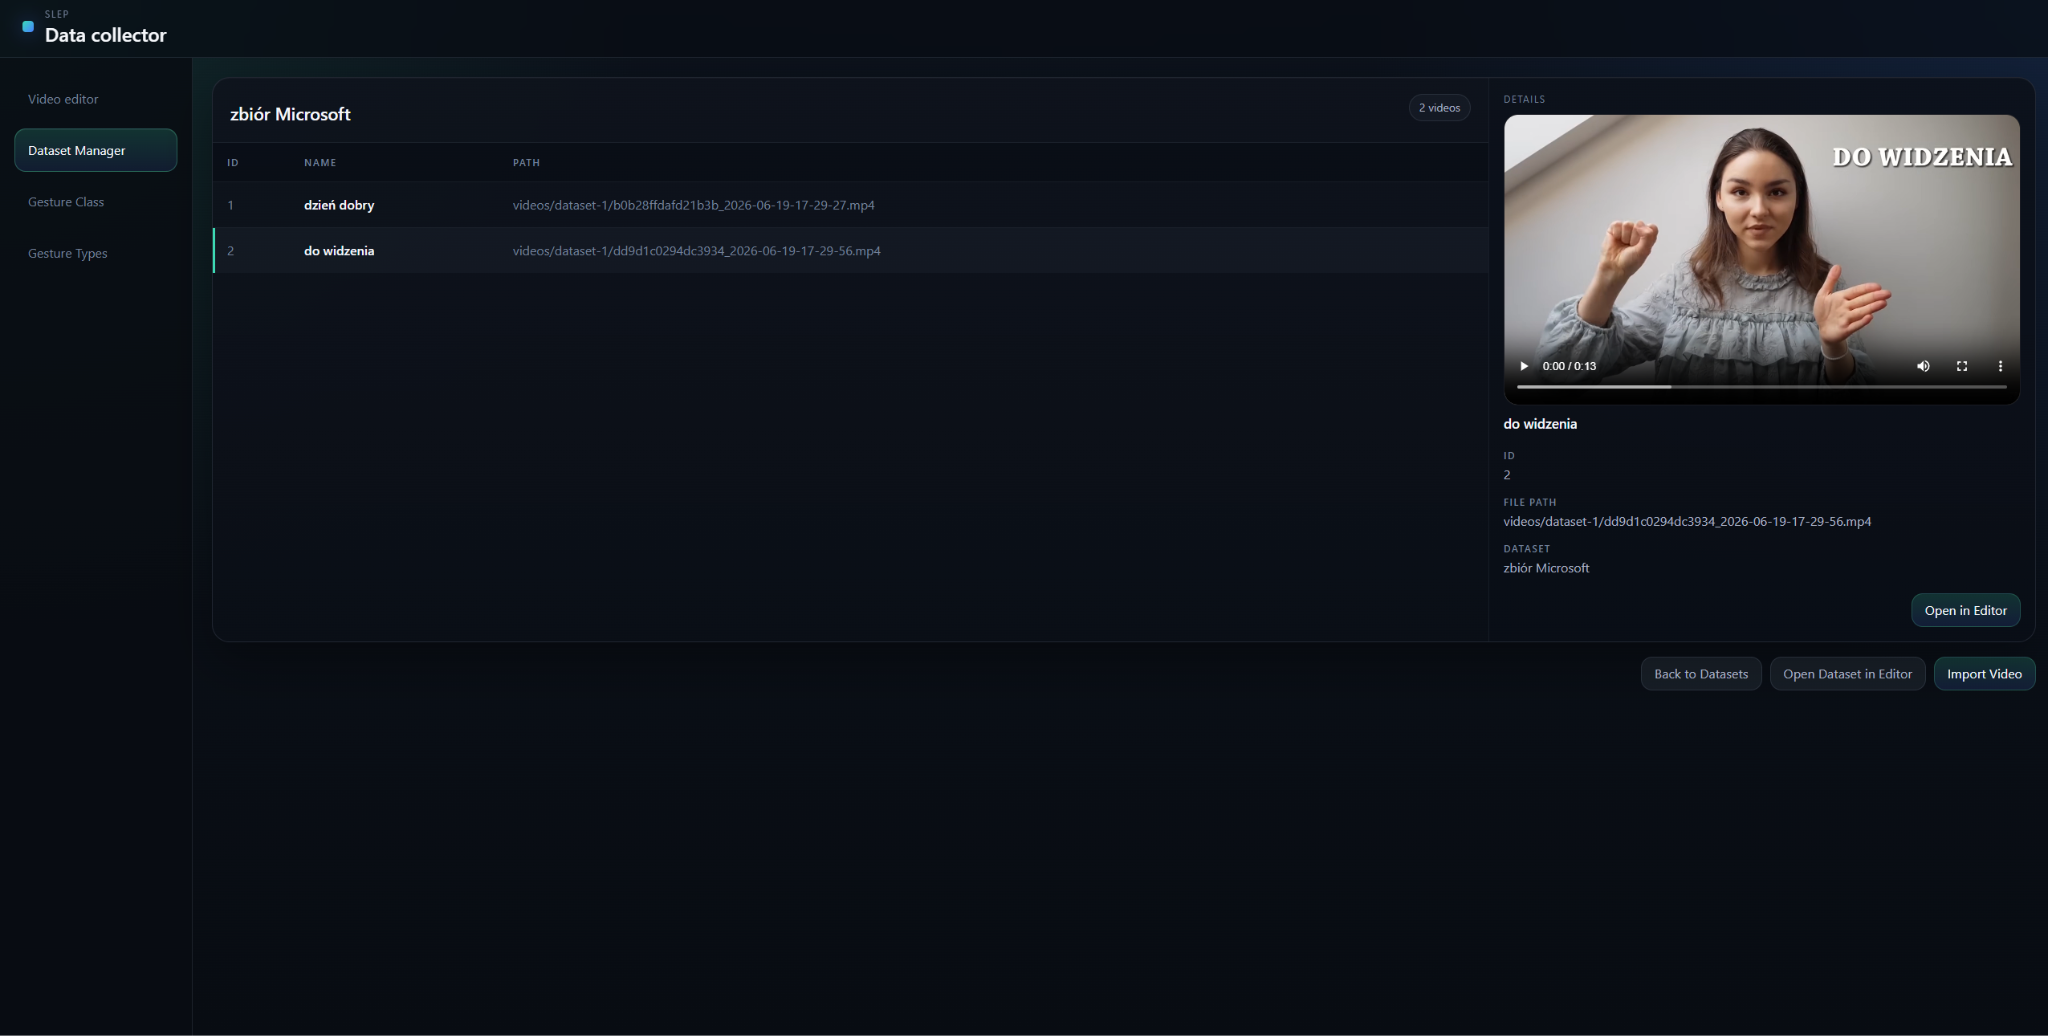
\includegraphics[width=0.85\textwidth]{figures/annotation-platform/dataset-videos-page.png}
  \caption{Dataset Manager's videos page.}
  \label{fig:dataset-videos-page}
\end{figure}

\begin{figure}[htbp]
  \centering
  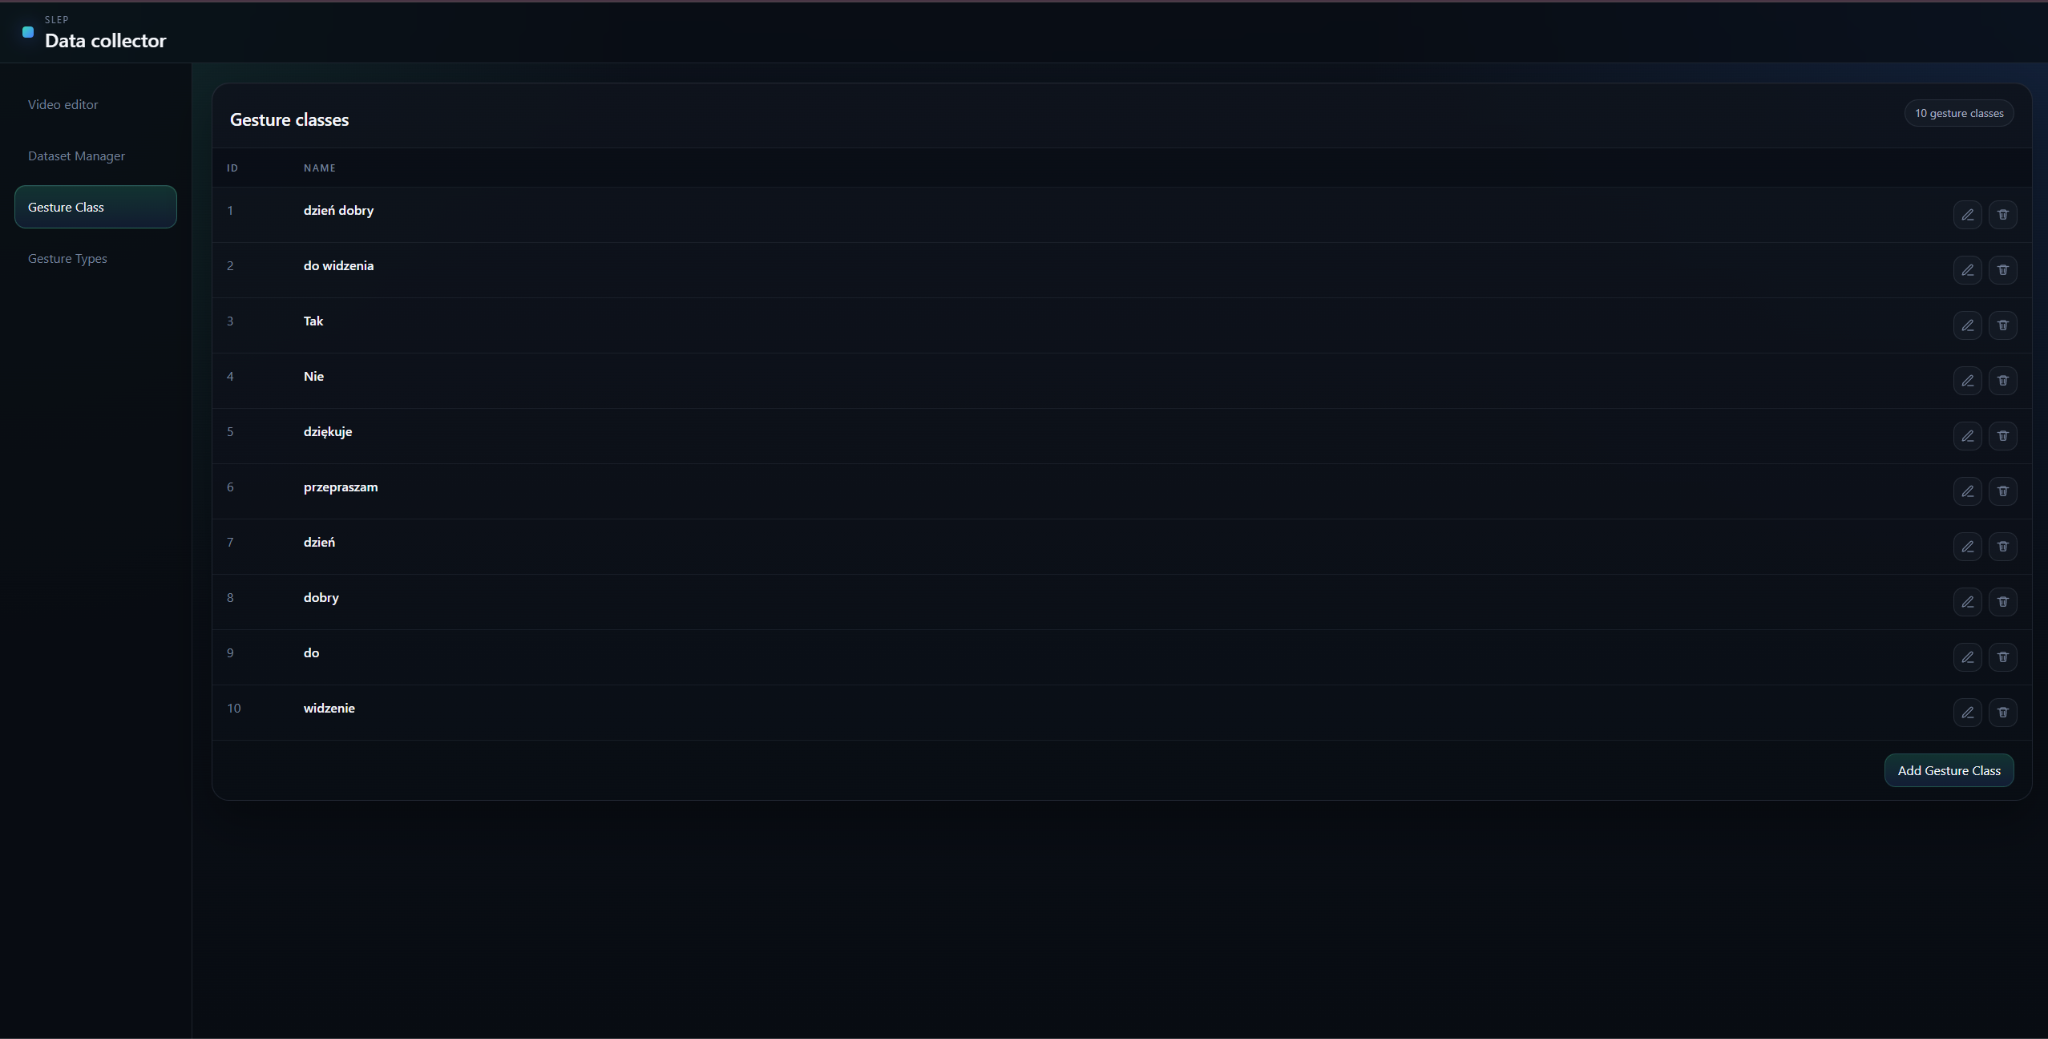
\includegraphics[width=0.7\textwidth]{figures/annotation-platform/gesture-classes-page.png}
  \caption{Gesture classes management page.}
  \label{fig:gesture-classes-page}
\end{figure}

\begin{figure}[htbp]
  \centering
  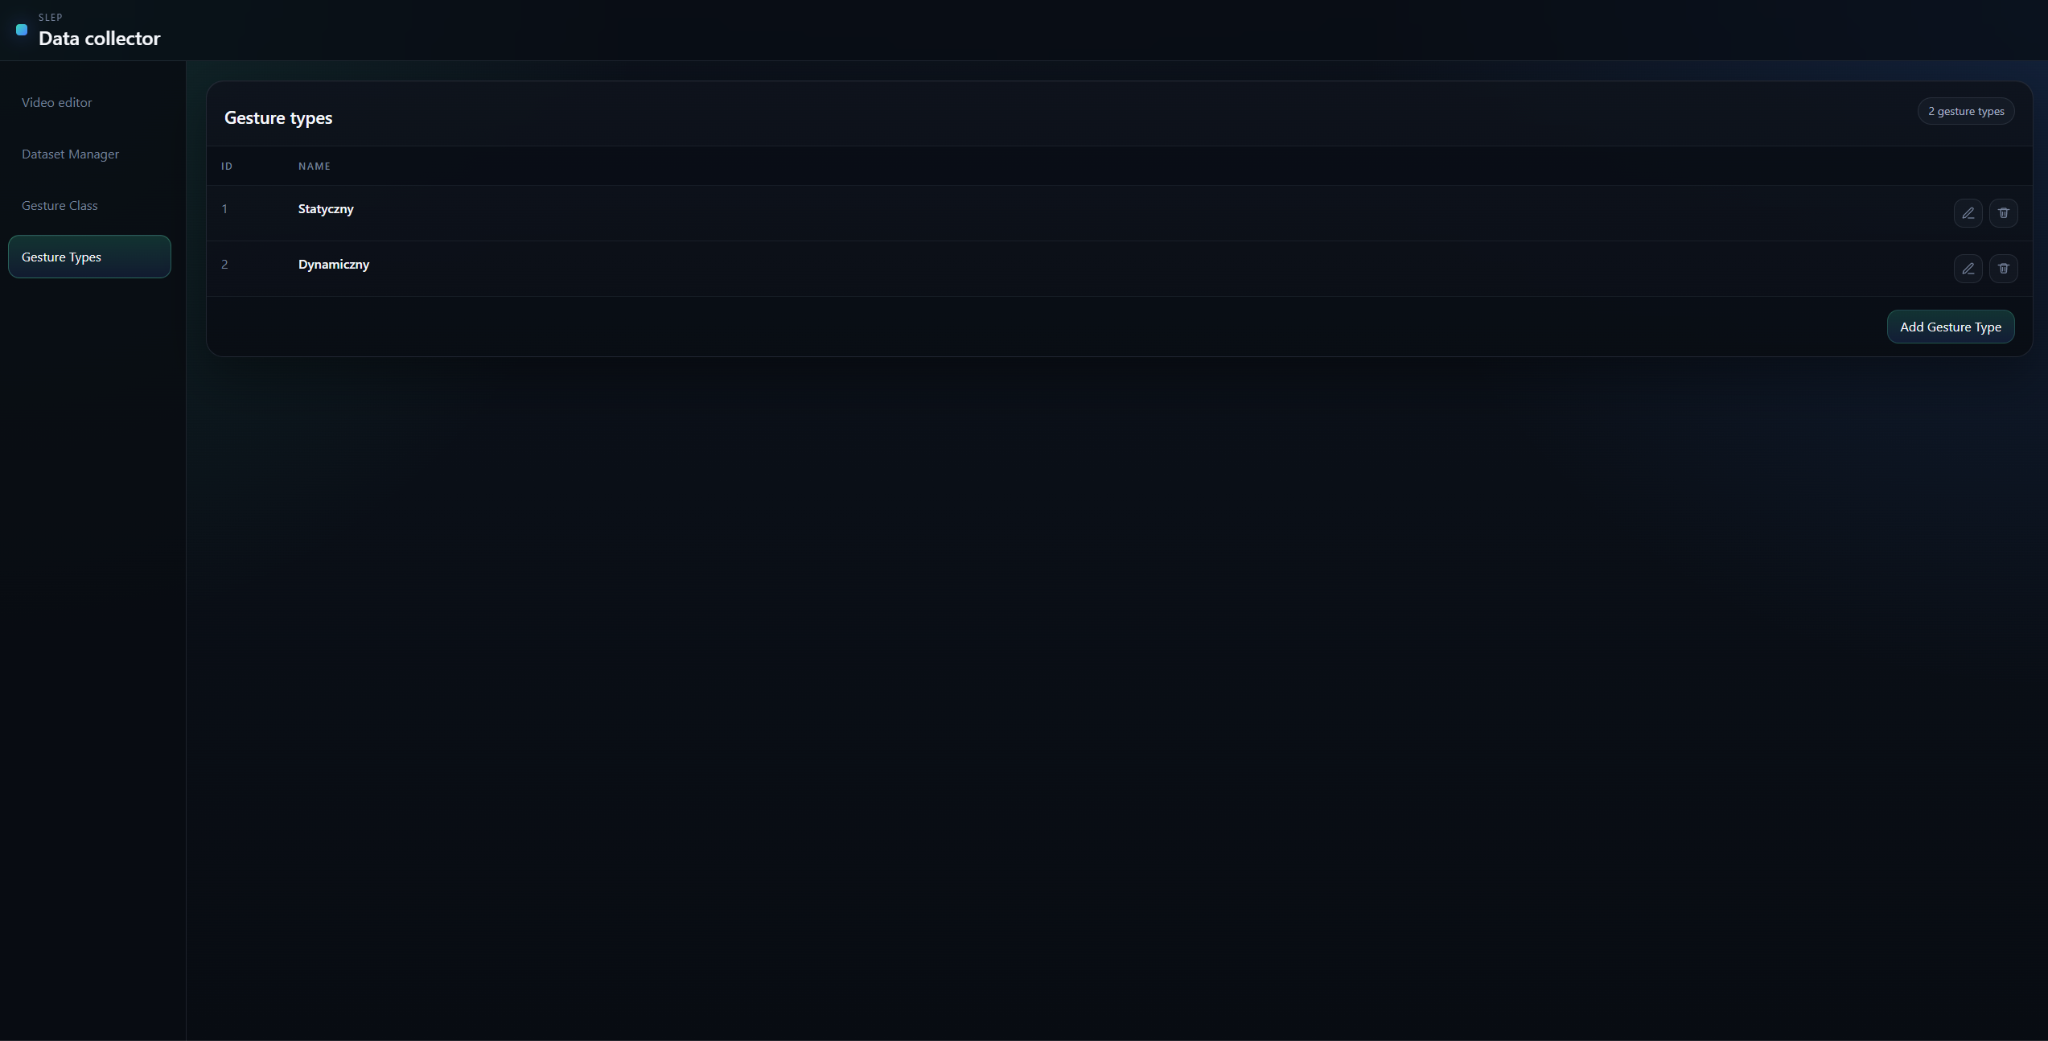
\includegraphics[width=0.7\textwidth]{figures/annotation-platform/gesture-types-page.png}
  \caption{Gesture types management page.}
  \label{fig:gesture-types-page}
\end{figure}

\subsection{System architecture}
\label{sec:annotation-system-architecture}

The application follows a typical full-stack architecture, illustrated in
Figure~\ref{fig:system-architecture}:

\begin{itemize}
  \item the React frontend handles user workflows and communicates with the
        backend through HTTP;
  \item the FastAPI backend exposes REST endpoints for datasets, videos,
        gesture metadata, import jobs, export jobs, and S3 signed URLs;
  \item PostgreSQL stores structured metadata, including datasets, videos,
        clips, landmarks, gesture classes, gesture types, and processing jobs;
  \item MinIO stores large binary files such as uploaded videos and generated
        landmark arrays;
  \item Redis acts as the Celery broker;
  \item Celery workers run long-running video processing tasks outside the
        request-response path.
\end{itemize}

This separation is important because video processing can be computationally
expensive. Uploading a video and requesting an import job returns control to the
web application quickly, while landmark extraction continues in the worker
process.

\begin{figure}[htbp]
  \centering
  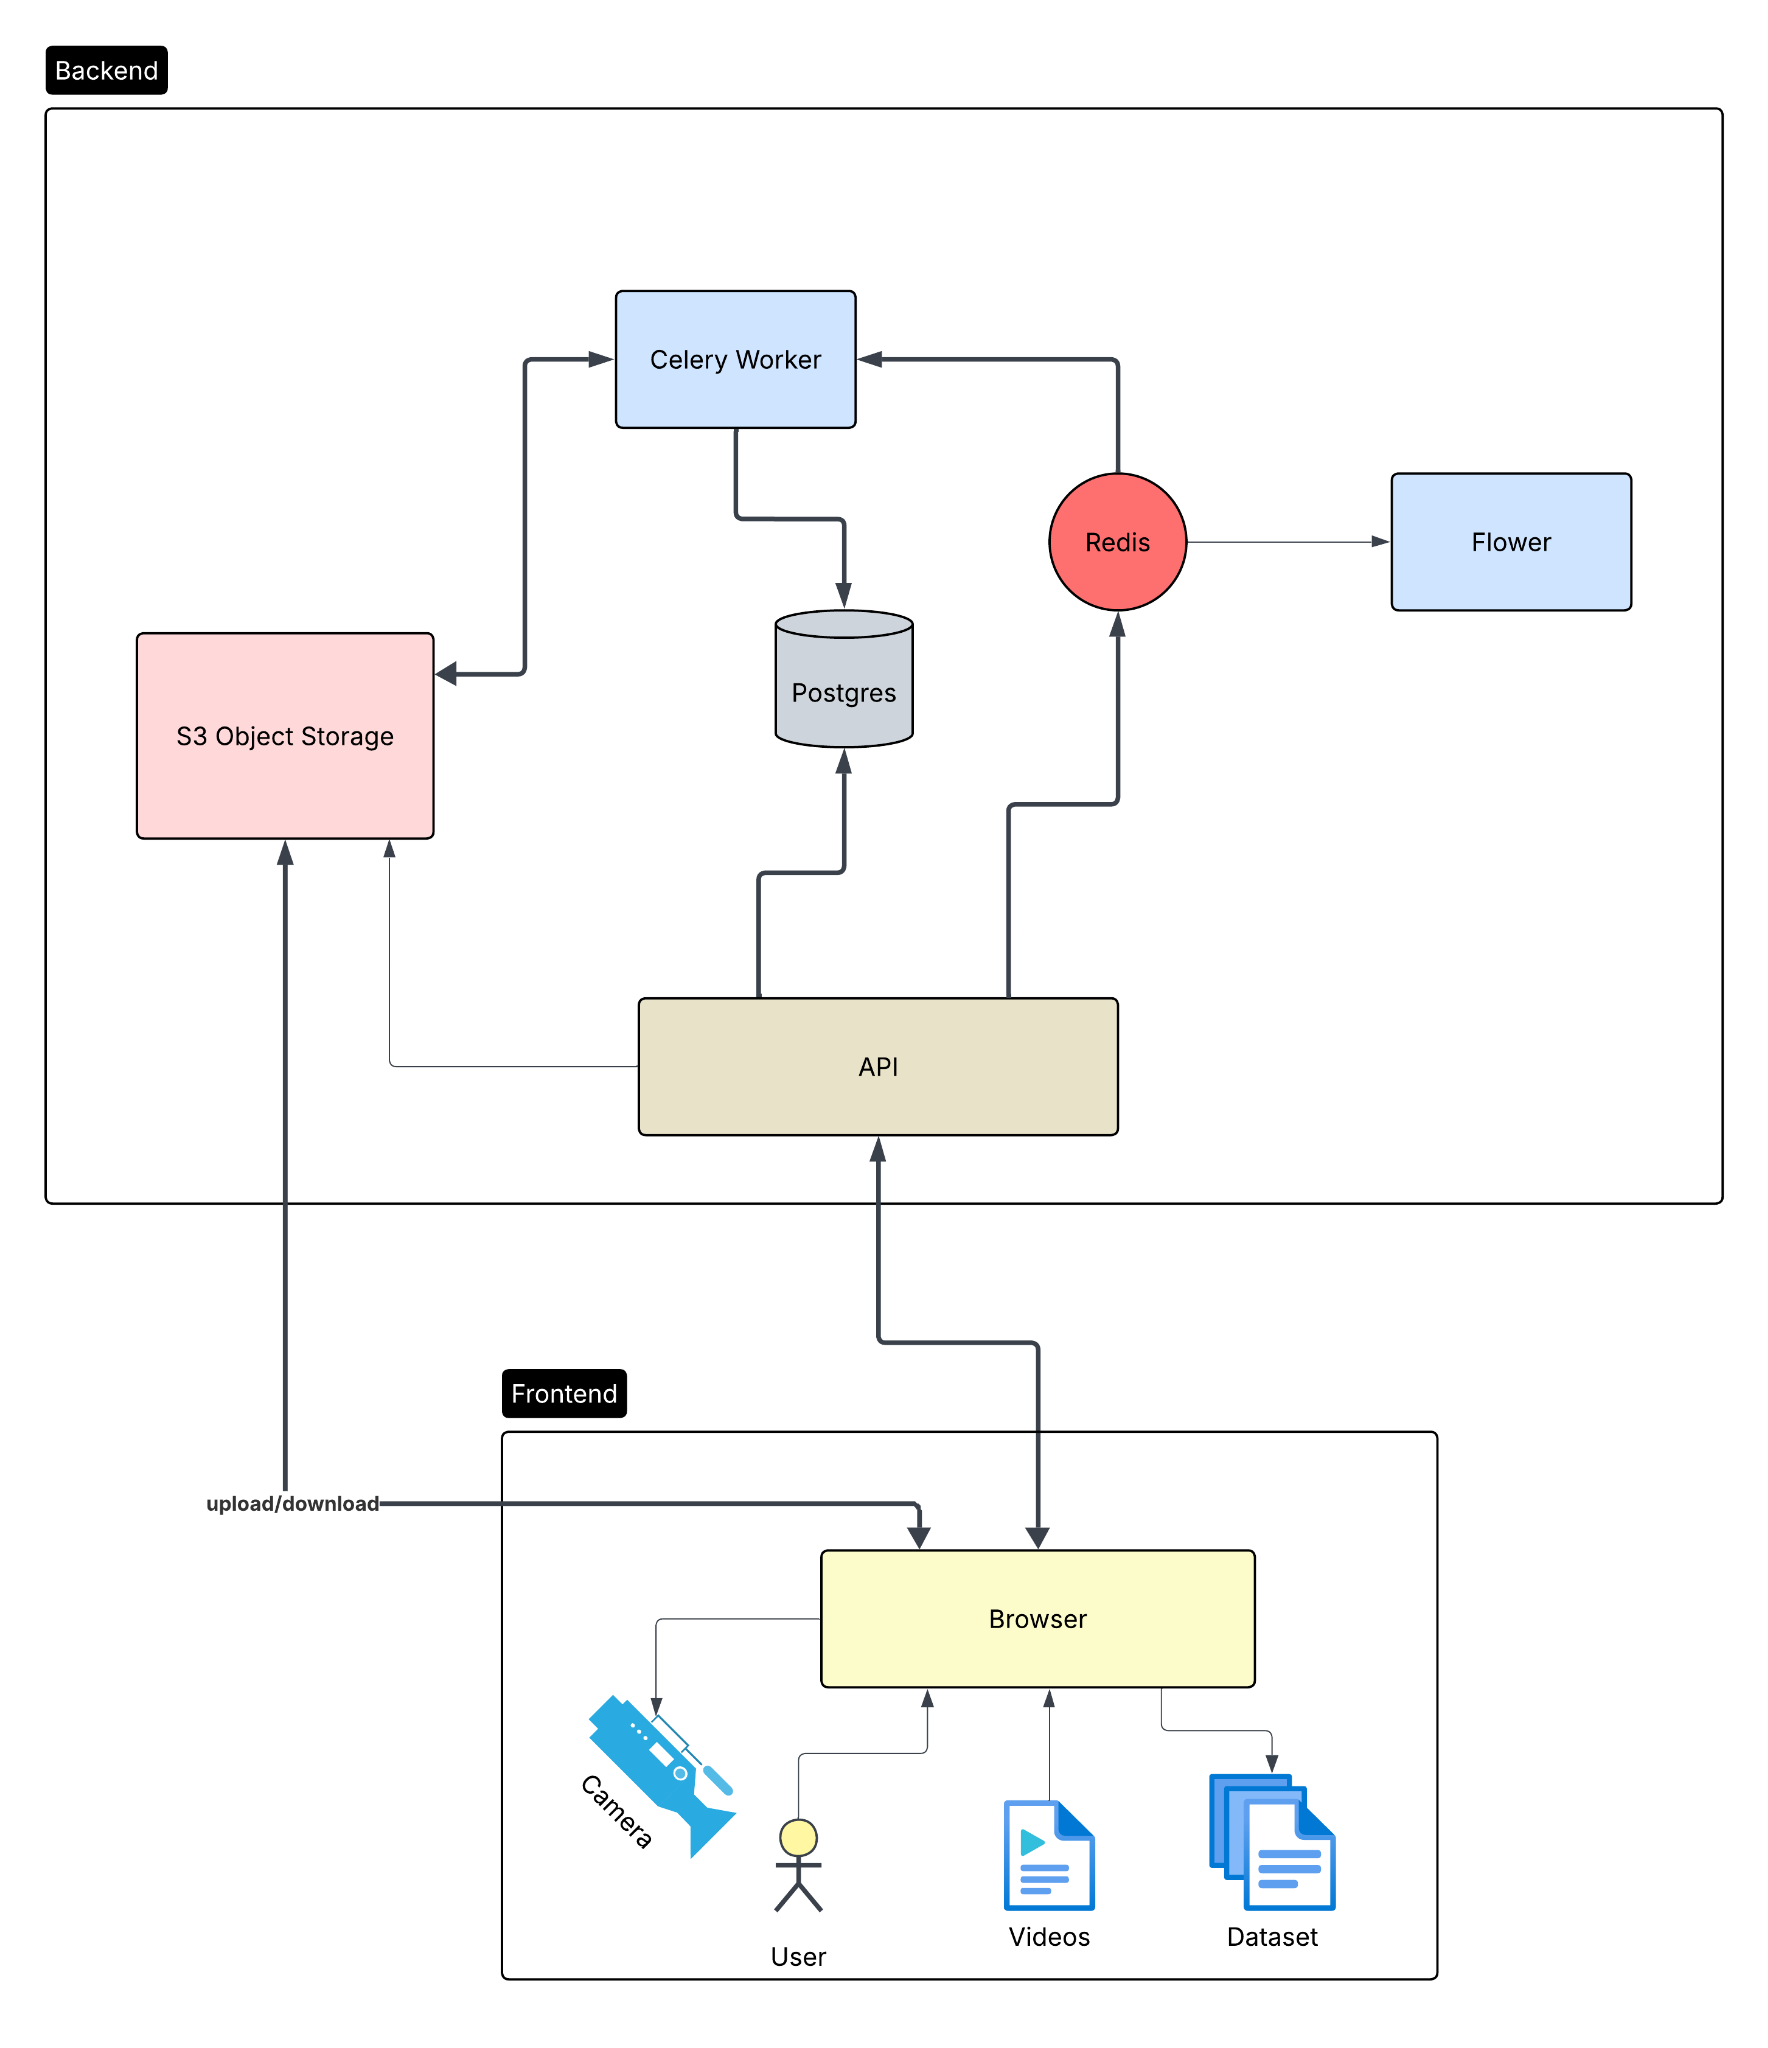
\includegraphics[width=0.85\textwidth]{figures/annotation-platform/system-architecture.png}
  \caption{Diagram of the annotation platform's system architecture.}
  \label{fig:system-architecture}
\end{figure}

The backend is implemented with Python~3.12, FastAPI, Pydantic, SQLAlchemy
async, Alembic, PostgreSQL, Redis, Celery, MinIO/S3, and MediaPipe. It exposes
REST endpoints under \texttt{/api/v1} and uses asynchronous database access for
application requests. It is organised around API routers, CRUD modules,
services, schemas, and SQLAlchemy models (Figure~\ref{fig:backend-structure}),
and implements the following API areas:

\begin{itemize}
  \item \textbf{datasets}: create, list, read, update, and delete datasets;
  \item \textbf{videos}: list videos, filter videos by dataset, read video
        details, update videos, delete videos, and manage related clips and
        landmarks;
  \item \textbf{gesture classes}: create, list, read, update, and delete
        gesture classes;
  \item \textbf{gesture types}: create, list, read, update, and delete gesture
        types;
  \item \textbf{import video jobs}: create and inspect video import jobs;
  \item \textbf{S3 integration}: generate signed upload and download URLs;
  \item \textbf{exported datasets and export dataset jobs}: database and API
        structures for future dataset export workflows.
\end{itemize}

\begin{figure}[htbp]
  \centering
  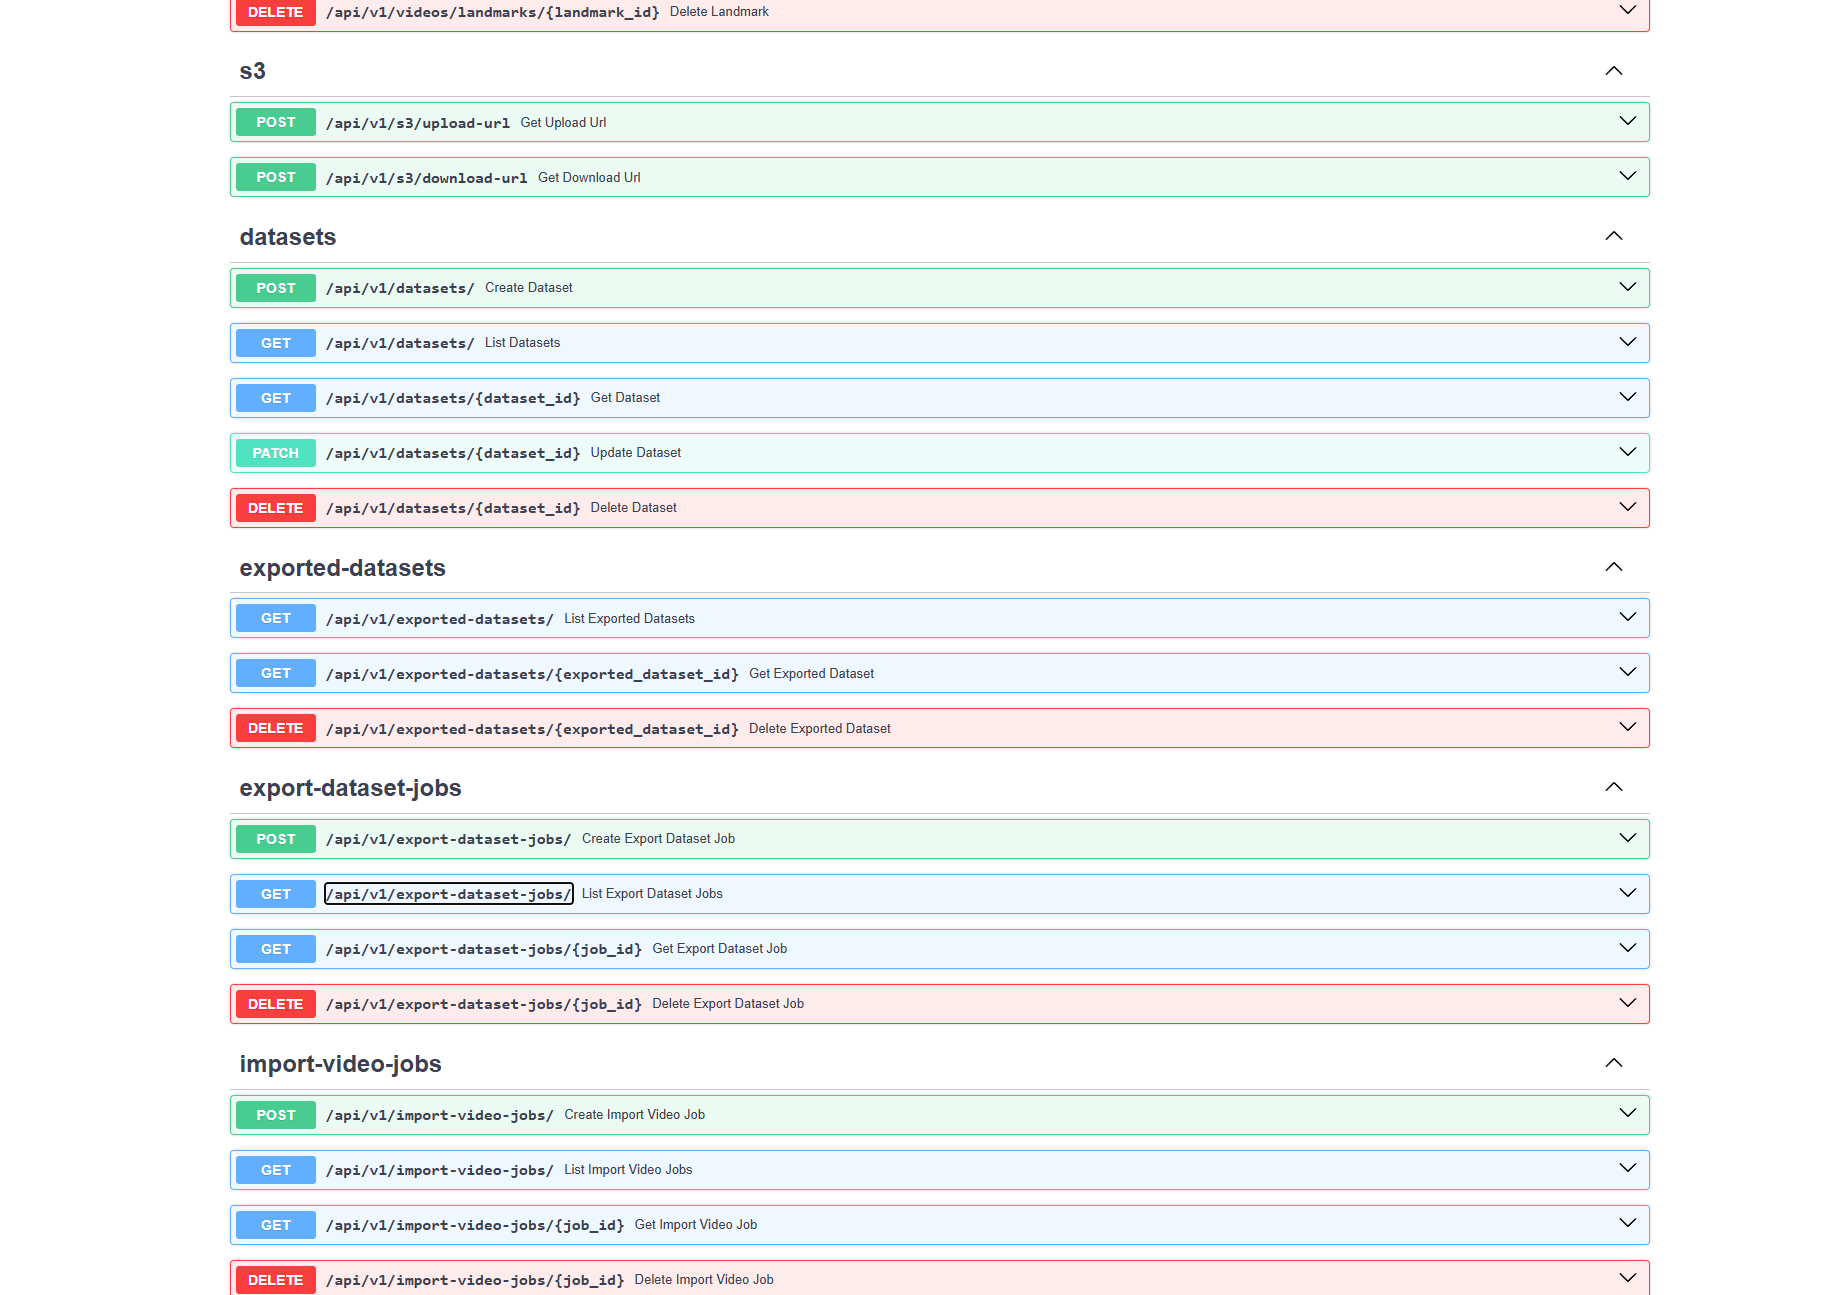
\includegraphics[width=0.7\textwidth]{figures/annotation-platform/swagger-ui.png}
  \caption{Backend API, Swagger UI.}
  \label{fig:swagger-ui}
\end{figure}

The import workflow is handled through \texttt{VideoService} and a Celery task.
When a video import job is created, the backend stores the job metadata and
dispatches a Celery task. The worker downloads the video from MinIO, extracts
landmarks, saves the result as a NumPy \texttt{.npy} file, uploads it back to
MinIO, creates a video record, and links the generated landmark file to that
video. The upload flow itself is implemented through signed S3 URLs: the
frontend asks the backend for an upload URL, uploads the selected file directly
to MinIO, and then creates an import job that references the uploaded object
path. This avoids sending large video files through the FastAPI application
process.

Video analysis is carried out asynchronously by a Celery worker
(task \texttt{process\_video}). The heart of the process is the
\texttt{LandmarkExtractionService}, which uses Google's MediaPipe Holistic and
proceeds as follows:

\begin{enumerate}
  \item \textbf{File retrieval} -- the service downloads the video file from
        the specified S3 key to the local worker environment;
  \item \textbf{ML network initialisation} -- the MediaPipe Holistic detector
        (\texttt{HolisticLandmarker}) is started via a context manager;
  \item \textbf{Frame-level extraction} -- detection runs on each video frame
        to extract spatial $x$, $y$, and $z$ coordinates;
  \item \textbf{Vectorisation} -- results for all components (face, body,
        hands) are combined into one flat vector, detailed in
        Section~\ref{sec:annotation-data-format};
  \item \textbf{Matrix aggregation} -- frame vectors are sequentially appended
        to a list, which ultimately becomes a 2D matrix of shape
        [number of frames $\times$ number of features];
  \item \textbf{Export to S3} -- the matrix is serialised as a \texttt{.npy}
        file (\texttt{numpy.save()}) and then uploaded to S3;
  \item \textbf{Database confirmation} -- a record is created in the
        \texttt{landmarks} table with the S3 key.
\end{enumerate}

For every frame, the landmark extraction service stores pose, face, left-hand,
and right-hand landmark coordinates in a fixed-size row; missing detections are
represented with zeros, which keeps the output array shape consistent across
frames and simplifies later machine learning use
(Figure~\ref{fig:annotation-methodology}).

\begin{figure}[htbp]
  \centering
  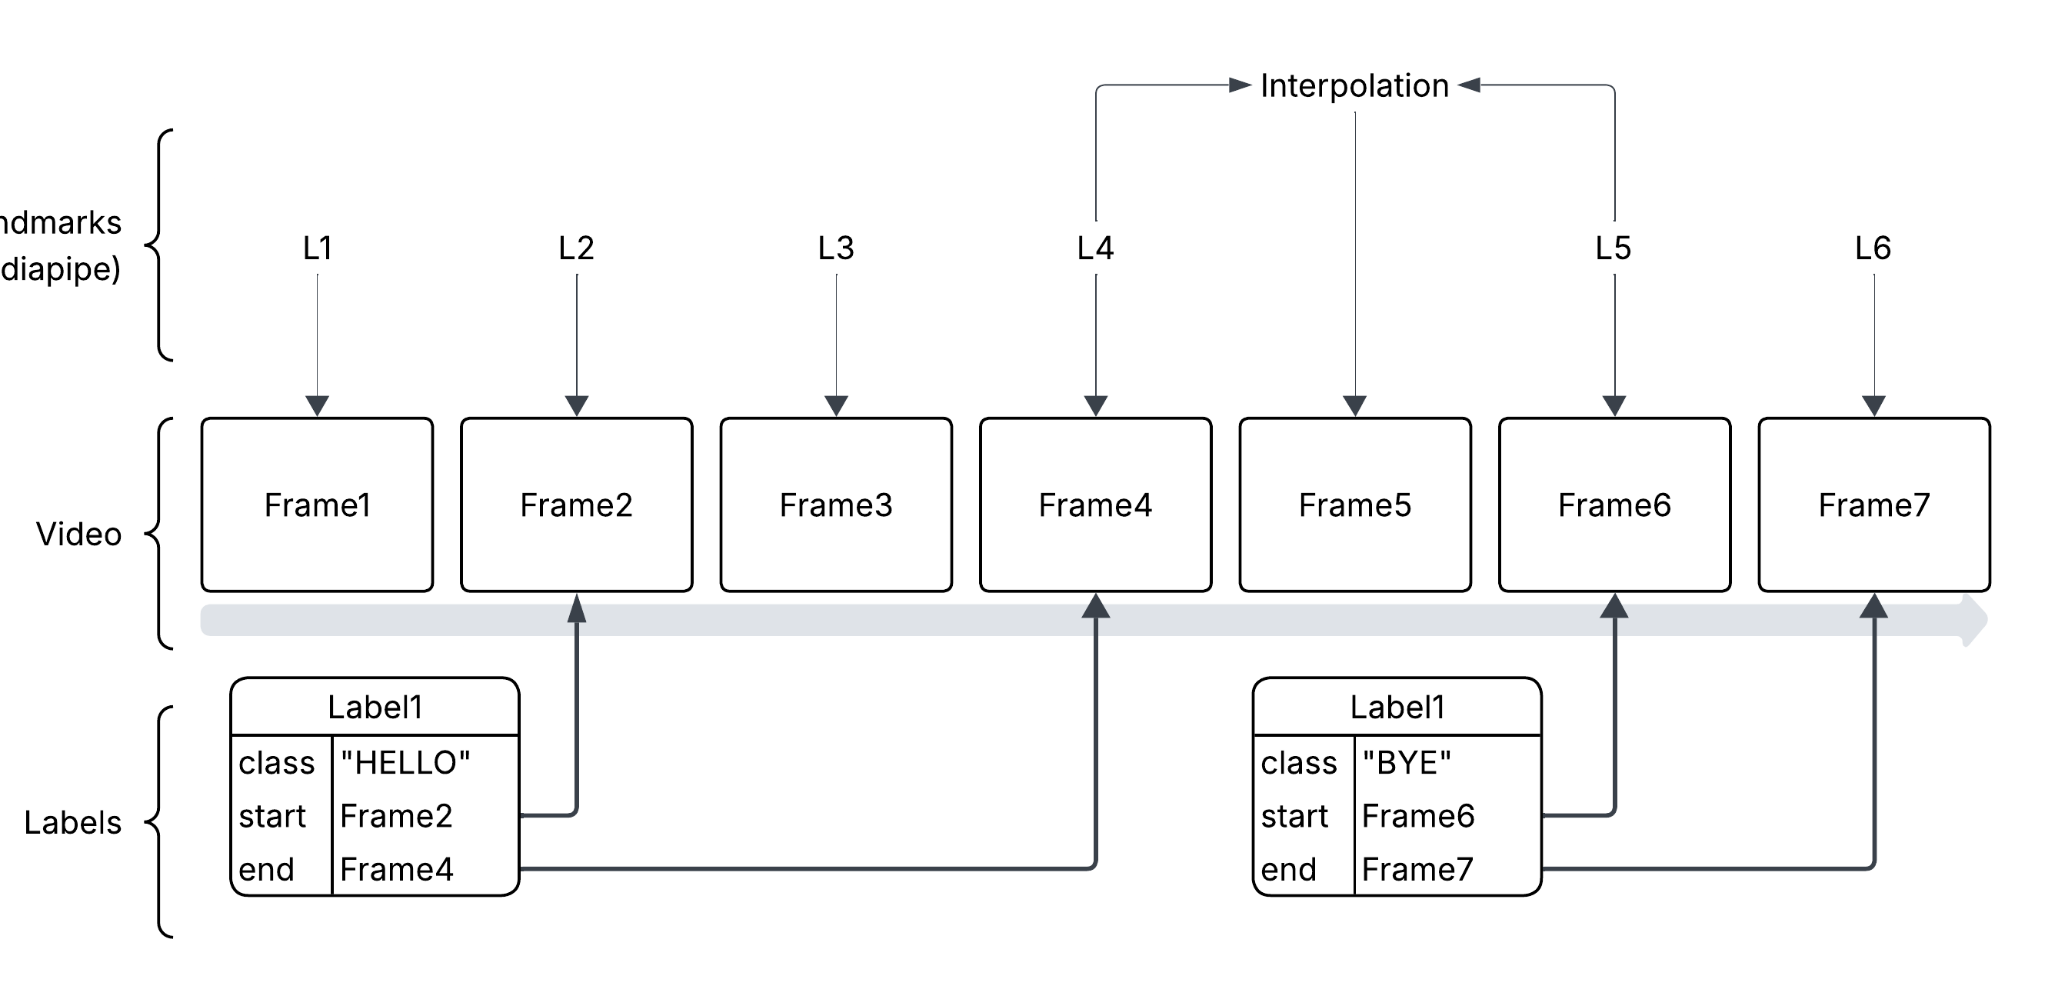
\includegraphics[width=0.85\textwidth]{figures/annotation-platform/annotation-methodology.png}
  \caption{Video-gloss annotation methodology.}
  \label{fig:annotation-methodology}
\end{figure}

The current database model contains the following main entities:

\begin{itemize}
  \item \textbf{Dataset} -- a named collection of related videos;
  \item \textbf{Video} -- metadata for a stored video, including file path,
        description, FPS, duration, and dataset relation;
  \item \textbf{Landmark} -- metadata for generated landmark files associated
        with videos;
  \item \textbf{Clip} -- an annotated frame range within a video;
  \item \textbf{GestureClass} -- a label category assigned to clips;
  \item \textbf{GestureType} -- an additional gesture classification assigned
        to clips;
  \item \textbf{ImportVideoJob} -- processing state for video import and
        landmark extraction;
  \item \textbf{ExportDatasetJob} -- processing state for future dataset export
        tasks;
  \item \textbf{ExportedDataset} -- metadata describing generated exported
        datasets.
\end{itemize}

The relationship between videos, clips, landmarks, gesture classes, and gesture
types creates a structured annotation layer over raw video data, suitable for
later dataset export and model training preparation. Key architectural
decisions made in the data model include:

\begin{itemize}
  \item \texttt{ON DELETE CASCADE} for related records (e.g.\ clips, landmarks,
        export dataset jobs) when the parent entity is deleted, eliminating
        orphaned data;
  \item \texttt{ON DELETE SET NULL} from datasets to videos: deleting a dataset
        does not delete its videos, it only sets \texttt{dataset\_id} to
        \texttt{NULL}, preserving valuable video data;
  \item \texttt{ENUM} types for job statuses (\texttt{in\_queue},
        \texttt{processing}, \texttt{done}, \texttt{error}), enforcing data
        consistency;
  \item denormalisation in \texttt{exported\_datasets}: dataset name and
        description are copied at export time, so the snapshot is immutable and
        the historical state of the dataset is always reproducible;
  \item separation of processing logic (\texttt{import\_video\_jobs},
        \texttt{export\_dataset\_jobs}) from business data (videos, clips,
        landmarks);
  \item separation of gesture semantics into \texttt{gesture\_classes} (general
        categories) and \texttt{gesture\_types} (specific types), allowing more
        flexible data modelling;
  \item nullable job fields (\texttt{video\_id}, \texttt{error\_message},
        \texttt{dataset\_id}, \texttt{exported\_dataset\_id}), allowing
        incremental record population during processing;
  \item no soft-delete mechanism: deleting an entity is a physical and
        irreversible operation.
\end{itemize}

The project includes Docker Compose services for the full development
environment: \texttt{postgres} for relational metadata storage, \texttt{redis}
for Celery queue communication, \texttt{s3-dev}/\texttt{s3} for MinIO object
storage, \texttt{data-collection-api} for the FastAPI backend,
\texttt{data-collection-worker} for background Celery processing,
\texttt{data-collection-flower} for monitoring Celery workers, and
\texttt{data-collection-frontend} for serving the frontend build through Nginx.
The frontend keeps API types and request functions in a shared actions module,
while pages and components focus on user workflows
(Figure~\ref{fig:frontend-structure}); the backend separates routers, schemas,
CRUD operations, services, models, and worker tasks
(Figure~\ref{fig:backend-structure}). Alembic migrations are present for
database schema evolution.

\begin{figure}[htbp]
  \centering
  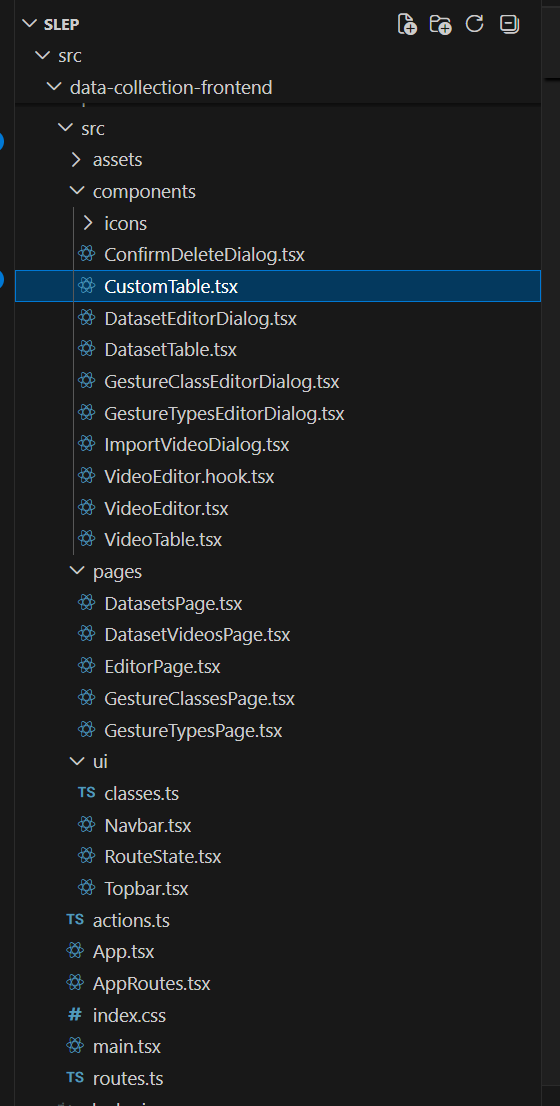
\includegraphics[width=0.6\textwidth]{figures/annotation-platform/frontend-structure.png}
  \caption{Frontend project structure.}
  \label{fig:frontend-structure}
\end{figure}

\begin{figure}[htbp]
  \centering
  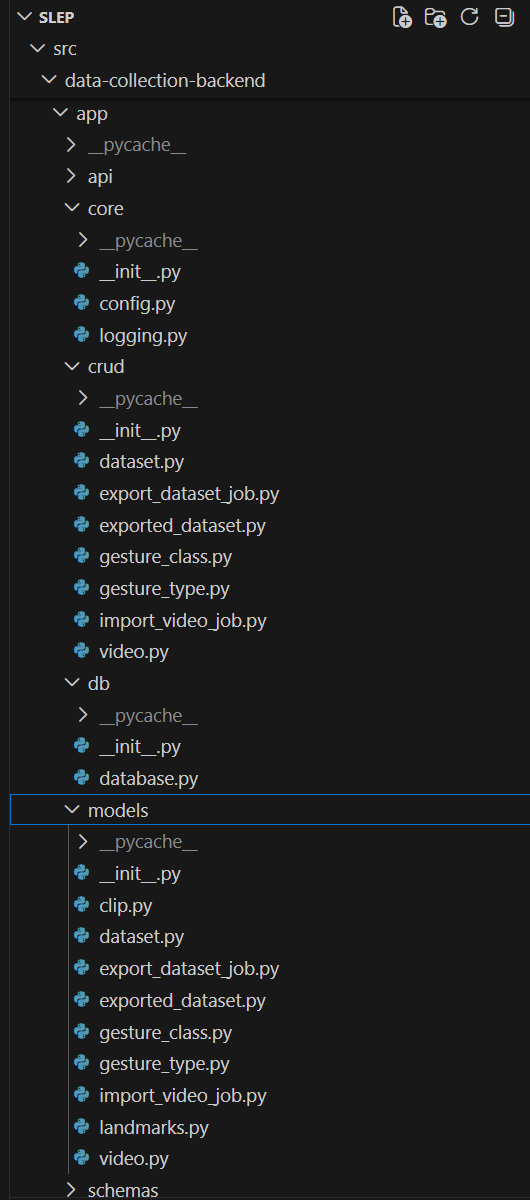
\includegraphics[width=0.5\textwidth]{figures/annotation-platform/backend-structure.png}
  \caption{Backend project structure.}
  \label{fig:backend-structure}
\end{figure}

\subsection{Data format and structure}
\label{sec:annotation-data-format}

Landmark files are stored in Amazon S3 as binary NumPy matrices (\texttt{.npy}).
Videos are addressed by an arbitrary S3 key, and their corresponding landmark
file uses the same key with a \texttt{\_landmarks.npy} suffix. Each \texttt{.npy}
file contains a 2D matrix with dimensions [number of video frames]
$\times$ [1659], as summarised in Table~\ref{tab:landmark-vector}.

\begin{table}[htbp]
  \centering
  \caption{Structure of the per-frame landmark feature vector (1659 values).}
  \label{tab:landmark-vector}
  \begin{tabular}{lccc}
    \hline
    \textbf{Component} & \textbf{Index range} & \textbf{Points} & \textbf{Values ($x,y,z$)} \\
    \hline
    Pose (silhouette) & 0--98    & 33  & 99   \\
    Face              & 99--1532 & 478 & 1434 \\
    Left hand         & 1533--1595 & 21 & 63  \\
    Right hand        & 1596--1658 & 21 & 63  \\
    \hline
    \textbf{Total}    & --       & 553 & 1659 \\
    \hline
  \end{tabular}
\end{table}

If a given element is not detected in a given frame (e.g.\ a missing right
hand), all of its assigned values are set to $0.0$. The resulting per-frame
representation -- one row per video frame, 1659 float32 columns per row -- is
the same landmark representation consumed by the preprocessing pipeline of the
isolated gloss recognition model described in
Section~\ref{sec:gloss-recognition-preprocessing}.

The end-to-end data flow through the platform proceeds in three stages:

\begin{enumerate}
  \item \textbf{Video import} -- a record is created in
        \texttt{import\_video\_jobs} with status \texttt{in\_queue}; the status
        is updated to \texttt{processing}; the file is downloaded and its
        metadata (FPS, duration) extracted; a record is created in
        \texttt{videos}; the job status is finally updated to \texttt{done}
        (with \texttt{video\_id} filled) or \texttt{error} (with
        \texttt{error\_message} filled);
  \item \textbf{Video processing (landmark extraction)} -- the Celery worker
        downloads the video from S3, runs MediaPipe Holistic on each frame,
        generates the landmark matrix and saves it to S3, creates a record in
        \texttt{landmarks}, and creates records in \texttt{clips} with
        \texttt{gesture\_class\_id} and \texttt{gesture\_type\_id} assignment;
  \item \textbf{Dataset export} -- a record is created in
        \texttt{export\_dataset\_jobs} with status \texttt{in\_queue}; the
        worker generates a data package (video and landmarks) for all videos in
        the dataset; a record is generated in \texttt{exported\_datasets} (with
        denormalised dataset data); the task status is updated to \texttt{done}
        or \texttt{error}.
\end{enumerate}

At the current stage, the project has a functional foundation for video dataset
management and annotation, supporting the complete path from dataset creation,
through video upload, to background landmark extraction and clip annotation.
The most developed areas are the backend CRUD and REST API structure, local
service orchestration with Docker Compose, S3-compatible video upload,
asynchronous landmark extraction through Celery, dataset and gesture taxonomy
management in the UI, and timeline-based clip annotation in the browser. The
dataset export workflow has database models, schemas, CRUD modules, and API
endpoints, but the asynchronous export processing pipeline still needs to be
completed, and import job status updates should be made more explicit throughout
the worker lifecycle.

Known limitations of the current platform include: video metadata such as FPS
and duration is currently stored with fixed values in the worker instead of
being fully derived from the uploaded file; the frontend API base URL is
hardcoded rather than configurable; authentication and authorisation are not
implemented; validation around clip ranges, duplicate labels, and dataset
consistency can be expanded; and landmark preview generation is modelled but not
fully implemented. Automated test coverage is also limited; the most important
future test areas are API endpoint behaviour, worker behaviour for successful
and failed imports, database migration validation, frontend editor behaviour for
frame selection and clip saving, and integration testing of the full
upload-import-processing path. These limitations do not prevent local data
collection experiments, but should be addressed before the platform is used as a
robust production or research data platform.

\todo{PLACEHOLDER: Insert an entity-relationship diagram summarising the
\texttt{datasets} / \texttt{videos} / \texttt{clips} / \texttt{landmarks} /
\texttt{gesture\_classes} / \texttt{gesture\_types} / \texttt{import\_video\_jobs}
/ \texttt{export\_dataset\_jobs} / \texttt{exported\_datasets} schema and its
foreign-key relationships.}
